Первый сцинтилляционный детектор назывался спинтарископом и был изобретён Уильямом Круксом в 1903 году. Главной его частью был небольшой экран, покрытый сульфидом цинка (ZnS). При попадании на него заряженных $\alpha$-частиц возникала слабая световая вспышка - сцинтилляция, которую можно было наблюдать в микроскоп или даже адаптированным к темноте невооружёным глазом.\par
В настоящее время сцинтилляционный детектор представляет собой устройство, содержащее кроме сцинтиллятора фотоприёмник и зарядочувствительный усилитель (ЗЧУ). Схема устройства представлена на рисунке ().\par
\begin{figure}[ht]
    \centering
    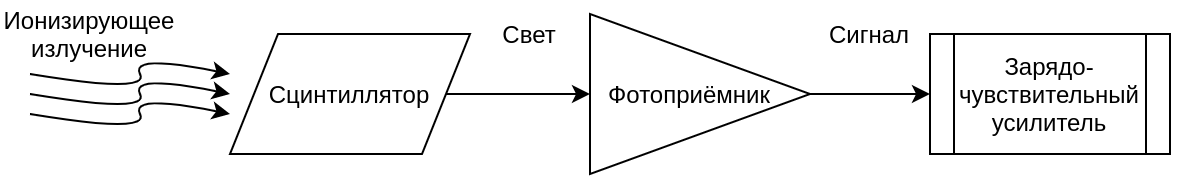
\includegraphics[width=1\linewidth]{Scintillation_detector.png}
    \caption{Схема сцинтилляционного детектора}
    \label{fig:mpr}
\end{figure}
Фотоприёмник преобразует излучённую кристаллом световую вспышку в импульс электрического тока. Полученный сигнал принимается ЗЧУ, который преобразует электрический ток в заряд. По величине заряда можно восстановить количество энегрии, потраченной сцинтиллятором на высвечивание за определённое время.
